\subsection{(R) Maneuverability Uncertainty Intersection}\label{s:uncertaintyIntersection}
\paragraph{Idea:} The \emph{intruders} are not bullets they are not sticking to predicted linear paths. The \emph{intruder} maneuverability is given as horizontal and vertical spread. Therefore \emph{intruder reach set} will form a \emph{elliptic cone}. This cone can be transformed into \emph{finite discrete } point-cloud, each \emph{point} should have assigned \emph{severity} impact value.  The point cloud intersection with  \emph{Avoidance Grid} will give us space impact of \emph{uncertain} intruder.


\begin{note}
    Following section will use condensed notation, due the equation complexity. The \emph{terminology} is consistent with rest of section. 
\end{note}

\paragraph{Sprace Intersection Rate - Body Volume Intersection:} $P_T(i_k({x}_s,{v},\theta,\varphi),c_{i,j,k})$
computation is less straight-forward than other space intersection rates. First let us define the linear intruder $i_k$ positions ${x}$ at time $t$ (eq. \ref{eq:vehiclelinearcone}) model, where ${x}(t)$ defines intruder position in \emph{avoidance grid euclidean coordinate frame} at time $t_i$, ${v}$ defines intruder velocity, and $t$ is time offset.

\begin{equation}\label{eq:vehiclelinearcone}
    x(t)=x_s + v_I.t
\end{equation}

\noindent Intruder \emph{horizontal spread} $\theta$ and \emph{vertical spread} $\varphi$ are introduced. These spreads represents intruder deviation limits along from linear trajectory prediction ${x}(t)\in\R^3$. The example is given by (fig. \ref{fig:P21ElipticConeIOnePoint}) where the intruder starts at point ${x}_s$ with fixed velocity $v$, the linear trajectory prediction is outlined by blue line. The \emph{predicted intruder position} at time $t=10s$ is given by ${x}(10)$ (blue point). The ellipsoidal space $E({x})$ is projected on the plane $D({x}(t))$. The plane $D$ (eq. \ref{eq:elisioidalOtrthogonalPlane}) for point ${x}(t)$ and velocity ${v}$ is defined as an orthogonal plane to velocity vector ${v}\in\R^3$ with origin at intruder position ${x}(t)$. 

\begin{equation}\label{eq:elisioidalOtrthogonalPlane}
    D({x}(t),{v})=\left\{{a}\in\R^3:({a}-{x}(t))\perp{v},\right\}
\end{equation}

To construct  ellipsoidal space boundary on orthogonal plane $D({x}(t),{v})$ some parameters are defined in (eq. \ref{eq:elipsiodialBoudaryParameters}). The \emph{scalar distance} $d_d{{x}(t)}$ is simple euclidean norm, \emph{maximal horizontal offset} $d_\theta({x}_t)$ is given as product of sinus of horizontal offset angle $\theta$ and scalar distance $d_d$, and \emph{maximal vertical offset} $d_\varphi({x}(t))$ is given a product of sinus of vertical offset angle $\varphi$ and scalar distance $d_d$.

\begin{equation}\label{eq:elipsiodialBoudaryParameters}
    \begin{aligned}
     d_d                      &=d_d({x}(t),{x}_s) =\norm{{x}(t)-{x}_s}_2\\ 
     d_{\theta_{\text{max}}}  &= d_\theta({x}(t))=\sin\theta   (i_k).d_d({x}(t))\\
     d_{\varphi_{\text{max}}} &= d_\varphi({x}(t))=\sin\varphi (i_k).d_d({x}(t)) 
    \end{aligned}
\end{equation}

\begin{figure}[H]
    \centering
    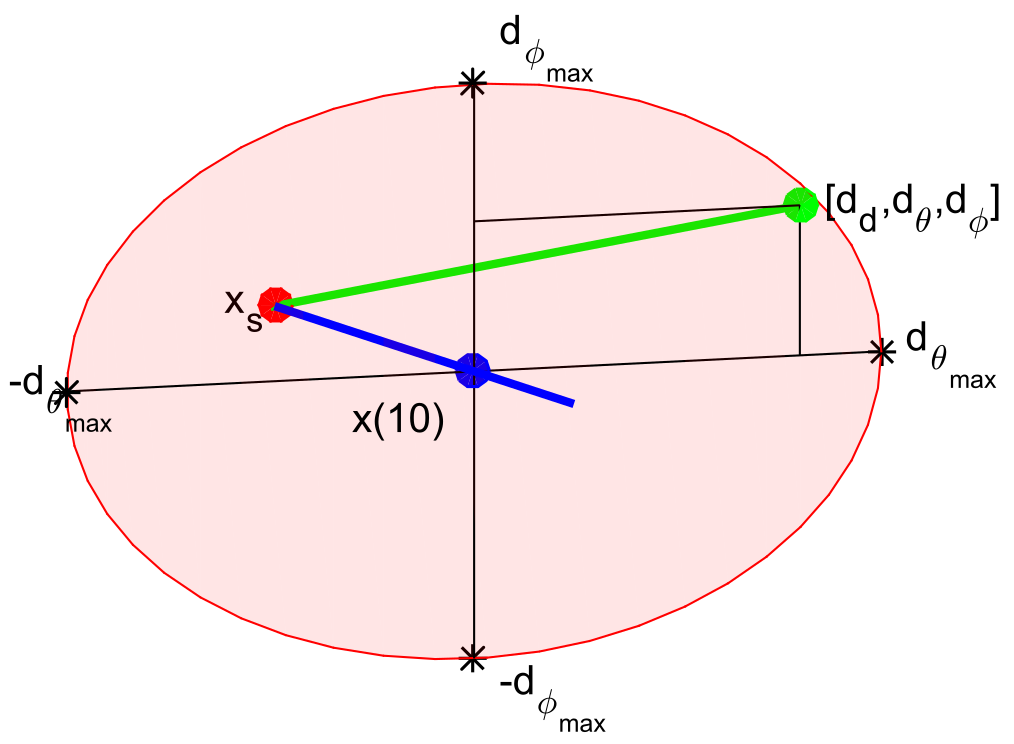
\includegraphics[width=0.7\textwidth]{\FIGDIR/TE014ElipticConeIOnePoint}         
    \caption{One rate position $[d_d,d_\theta,d_\varphi]$ (green). deviated from linear trajectory (blue line) at point ${x}(10)$.(blue) with initial position $x_s$ (red)}
    \label{fig:P21ElipticConeIOnePoint}
\end{figure}

\noindent The \emph{Ellipsoid} $E({x}(t),{v})$ (eq. \ref{eq:baseElipsoidxt}) for fixed intruder position ${x}(t)$ and fixed intruder velocity ${v}$ is given as constrained portion of orthogonal plane $D({x}(t),{v})$. The constraint is defined by an internal coordinate frame ${p}\in \R^2$ which is space reduction of plane $D({x}(t),{v})$. 

The internal coordinate frame ${p}\in\R^2$ has origin in ${x}(t)\to\R^2$. The points of plane ${p}$ are bounded by projection ${p}=({b}-{x}(t))\to\R^2$, where $b\in D({x}(t),v)$. The point of ellipsoidal ${p}$ is then given as standard ellipse boundary with vertical span $d_\theta({x}(t))$ and horizontal span $d_\varphi({x}(t))$. 

The 2D \emph{Ellipsoid} $E({x}(t),{v})$ for specific time $t=10s$ example is portrayed  as red ellipsoid (in fig. \ref{fig:P21ElipticConeIOnePoint}).

\begin{equation}\label{eq:baseElipsoidxt}
    E({x}(t),{v})=\left\{ \begin{aligned}{b}\in\R^3:&{b}\in D({x}(t),{v}),{p}=({b}-{x}(t))\to\R^2,\\&\left(\frac{p(1)^2} {d_\theta({x}(t))^2}+ \frac{p(2)^2}{d_\varphi({x}(t))^2}\right)\le 1\end{aligned}\right\}
\end{equation}

\noindent The expected behaviour of an intruder $i_k$ is to stick to predicted linear trajectory ${x}(t)$ (\ref{eq:vehiclelinearcone}). The probability of deviation should be decreasing with distance from ellipse center (fig. \ref{fig:intruderPassingProbability}.).  
\begin{figure}[H]
    \centering
    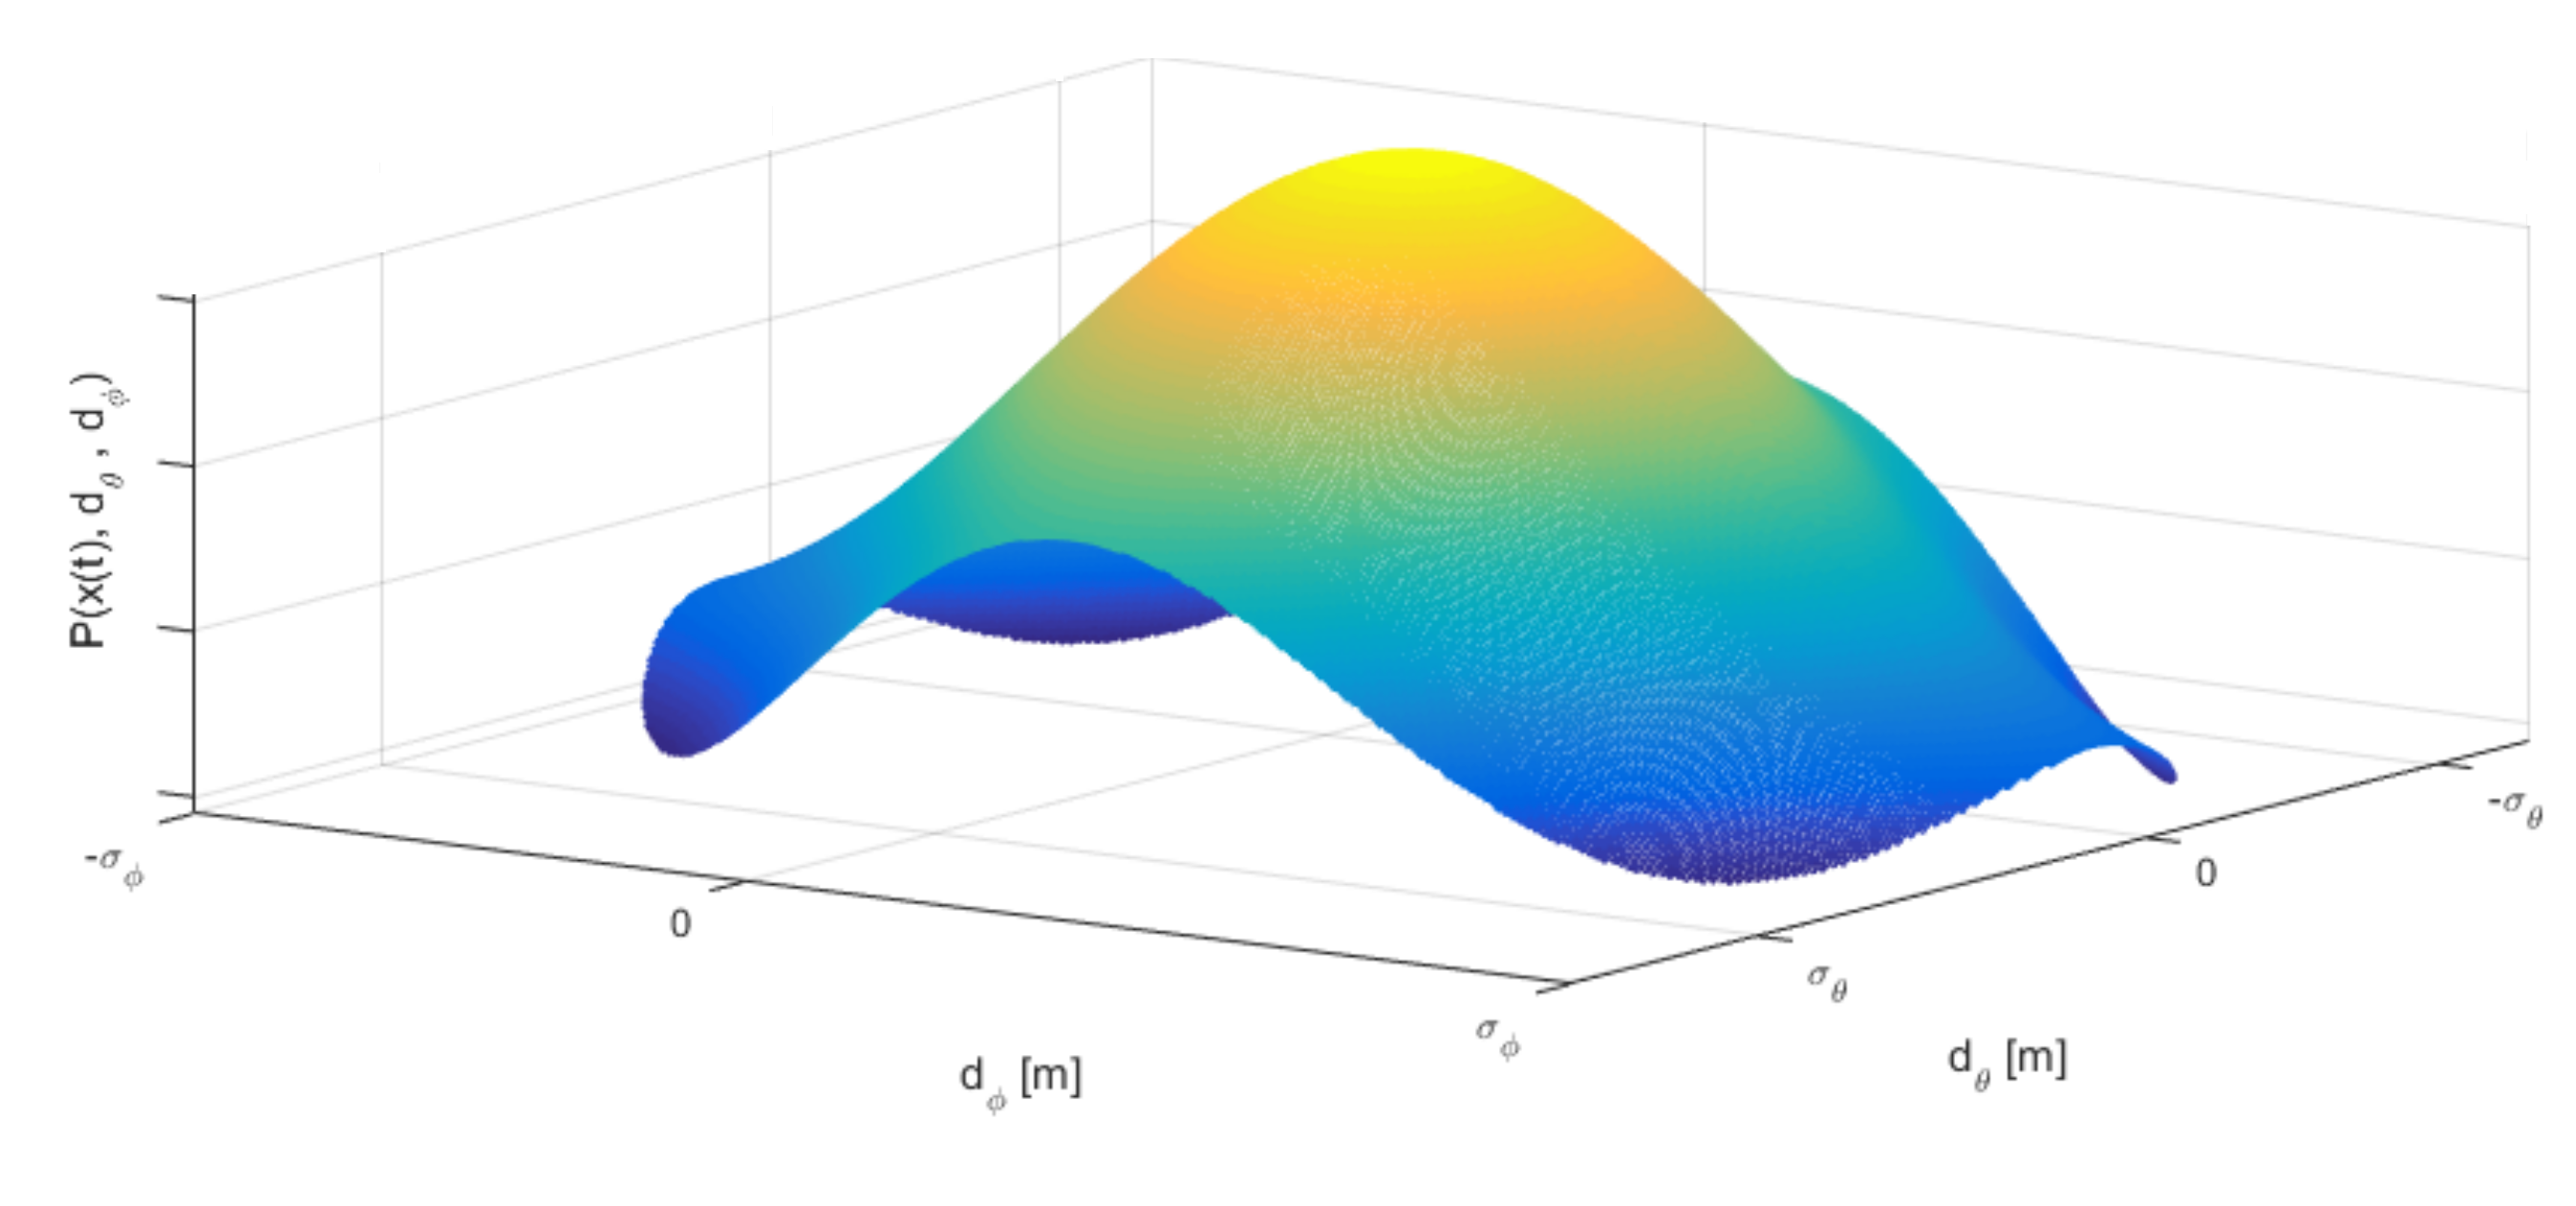
\includegraphics[width=0.9\textwidth]{\FIGDIR/TE015ProbabilisticDistributionOfEllipsoidCutSideForTE016}
    \caption{Probability of intruder $i_k$ position in ellipsoid $E({x}(t),{v})$}
    \label{fig:intruderPassingProbability}
\end{figure}

\noindent \emph{Probability density function} for ellipsoid  $E({x}(t),{v})$defined in (eq. \ref{eq:baseElipsoidxt}) is depending on maximal horizontal spread $d_\theta({x}(t))$, maximal vertical spread $d_\varphi({x}(t))$, defined by (eq. \ref{eq:elipsiodialBoudaryParameters}). 

Two standard probabilistic distributions are established $\mathscr{N}(\mu_\theta,\sigma_\theta)$ (eq. \ref{eq:elipsprobdistHorizontal}) for horizontal spread $\theta({x}(t))$ and $\mathscr{N}(\mu_\varphi,\sigma_\varphi)$  (eq. \ref{eq:elipsprobdistVertical}) for vertical spread $\varphi({x}(t))$. The means $\mu_\theta$ and $\mu_\varphi$ are set to zero, and internal coordinate frame ${p}\in\R^2$ where ${x}(t)\to\R^2$ is frame center. The variances $\sigma_\theta$ and $\sigma_\varphi$ are set as maximal distances on horizontal/vertical spread axes $d_\theta({x}(t))$ and $d_\varphi({x}(t))$.

\begin{equation}\label{eq:elipsprobdistHorizontal}
    P({x}(t),d_\theta)=\mathscr{N}(\mu_\theta,\sigma_\theta)=\mathscr{N}(0,d_\theta({x}(t)))
\end{equation}

\begin{equation}\label{eq:elipsprobdistVertical}
    P({x}(t),d_\varphi)=\mathscr{N}(\mu_\varphi,\sigma_\varphi)=\mathscr{N}(0,d_\varphi({x}(t)))
\end{equation}

\noindent The combined \emph{probability density function} for maximal spreads $d_\theta$ and $d_\varphi$ is given by (eq. \ref{eq:elipsprobdistCombined}). Because probability density function is defined for internal space ${p}\in\R^2$ and one may need to calculate impact rate for  cell space $c_{i,j,k}\in\R^3$. 

The reduction from two parameter probability distribution function to scalar rate distribution function is needed. An scalar rate distribution  function $P({x}(t),d_\theta,d_\varphi)$ over ellipsoid $E({x}(t),{v})$ is defined as (eq.\ref{eq:elipsprobdistCombined}), where final rate is given as average of two partial probabilities. 

Final space intersection rate $P({x}(t),d_\theta,d_\varphi)$ needs to be normalized to hold \emph{normal distribution condition} (eq. \ref{eq:normalDistrobitionCondition}). Normal distribution condition value (eq. \ref{eq:normalDistrobitionCondition}) is given as surface integral over ellipsoid $E({x}(0),{v})$ with rate distribution function $P({x}(t),d_\theta,d_\varphi)$.

\begin{equation}\label{eq:elipsprobdistCombined}
    P({x}(t),d_\theta,d_\varphi) = \frac{\mathscr{N}(\mu_\theta,\sigma_\theta)+\mathscr{N}(\mu_\varphi,\sigma_\varphi)}{2}
\end{equation}

\begin{equation}\label{eq:normalDistrobitionCondition}
    \iint_{E({x}(\tau))} P({x}(t),d_\theta,d_\varphi) \,\text{d}d_\theta\,\text{d}d_\varphi = 1
\end{equation}

\noindent Final space intersection rate  $P({x}(t),c_{i,j,k},\theta,\varphi)$  (space portion, time portion is calculated in (eq.\ref{eq:intruderIntersectionProbability}) is given by (eq. \ref{eq:spreadIntruderIntersectionProb}). Its mean value of all intersection rates $P({x}(\tau),c_{i,j,k},\theta,\varphi)$ where $\tau\in[i_e(c_{i,j,k}),i_l(c_{i,j,k})]$ is fixed point in intersection time interval.

An $P({x}(\tau),c_{i,j,k},\theta,\varphi)$ (\ref{eq:spreadIntersectionProbFixedtau}) is integration of rate density function $P({x}(\tau),d_\theta,d_\varphi)$ (eq. \ref{eq:elipsprobdistCombined}) in surface $E({x}(\tau),{v})$ to cell $c_{i,j,k}$ volume intersection. 

To get a volume integration partial rate in surface intersection must be integrated and normalized in time interval $\tau\in[i_e(c_{i,j,k}),i_l(c_{i,j,k})]$, the \emph{base intersection probability} $P_T(i_k({x}_s,{v},\theta,\varphi),c_{i,j,k})$ is given by (eq. \ref{eq:spreadIntruderIntersectionProb}). Example of intersection of intruder $i_r$ uncertain ellipsoid cone with avoidance grid $\mathscr{A}(t_i)$ is given in (fig. \ref{fig:ellipticConeIntersectionExample}).

\begin{equation}\label{eq:spreadIntersectionProbFixedtau}
    P({x}(\tau),c_{i,j,k},\theta,\varphi) =\iint_{E({x}(\tau),{v})\cap c_{i,j,k}} P({x}(\tau),d_\theta,d_\varphi)
\end{equation}

\begin{equation}\label{eq:spreadIntruderIntersectionProb}
    P_T(i_k({x}_s,{v},\theta,\varphi),c_{i,j,k})=\frac{\int_{i_e(c_{i,j,k})}^{i_l(c_{i,j,k})} P({x}(\tau),c_{i,j,k},\theta,\varphi)\,\text{d}\tau}{i_l(c_{i,j,k})-i_e(c_{i,j,k})}
\end{equation}

\begin{figure}[H]
    \centering
    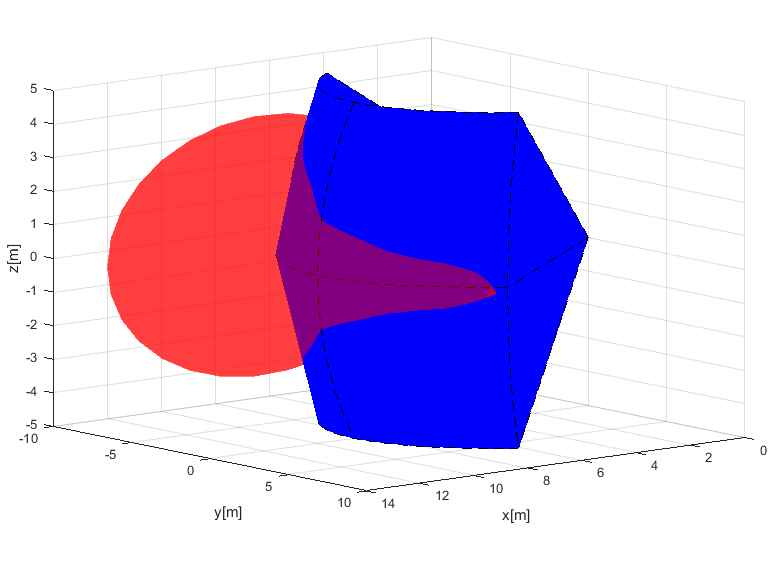
\includegraphics[width=0.7\textwidth]{\FIGDIR/TE013ElipticConeIntersecitonExample}
    \caption{Avoidance grid $\mathscr{A}(t_i)$ (blue) intersection with elliptic cone intruder $i_k({x},{v},\theta,\varphi)$ (red) example.}
    \label{fig:ellipticConeIntersectionExample}
\end{figure}

\noindent An \emph{numeric approximation} of space intersection rate $P_T(i_k({x}_s,{v},\theta,\varphi),c_{i,j,k})$ is more implementation feasible than symbolic calculation due the multiple intersection constraints and bad intersection algorithm complexity. 

Let us define homogeneous discrete subset of real numbers $\mathscr{R}$ which is non empty subset of real numbers $\R$. The set $\mathscr{R}$ (eq. \ref{eq:homogeneusdiscretizationofRealnumbers}) is homogeneous, that means for any equal interval $(i,i+1],i\in\mathbb{Z}$ subset the count of members is equal to some positive natural number $k$. The parameter $k$ can be understand as \emph{unit approximation density}.

Similarly the power sets $\mathscr{R}^2\subset\R^2$, $\mathscr{R}^3\subset\R^3$, ... $\mathscr{R}^i\subset\R^i,i\in\N^+$ keeps homogeneous distribution.

\begin{equation}\label{eq:homogeneusdiscretizationofRealnumbers}
    \mathscr{R} = \left\{\begin{aligned}a\in\R:&\forall i\in\mathbb{Z},|i<a\le i+1|=k,k\in\N^+, \\&\forall j\in \N^+a_{j+1}-a_{j}=m,m\in\R^+\end{aligned}\right\},\,\mathscr{R}\subset\mathbb{R}
\end{equation}

\noindent The orthogonal plane for ${x}(t), {v}, t \in\R$ is defined by (eq. \ref{eq:elisioidalOtrthogonalPlane}). The orthogonality property is also kept for any subspace $\mathscr{R}^n\in\R^n,n\in\N^+$. Numeric approximation of $D({x}(t),{v})$ is given as $D_D({x}(t),{v})$ (eq. \ref{eq:elisioidalOtrthogonalPlaneDiscrete}). 

The only difference is that discrete approximation is countable $|D_D|=m,m\in\N^+$, but continuous representation $|D|\approx \infty$ is uncountable. Because ellipsoid is subset of orthogonal plane it keep its countability property, therefore $E_D$ is also countable and must contains at-least one member.

\begin{equation}\label{eq:elisioidalOtrthogonalPlaneDiscrete}
    D_D({x}(t),{v})=\left\{{a}\in\mathscr{R}^3:({a}-{x}(t))\perp{v},\right\},t\in\mathscr{R}
\end{equation}

\noindent The \emph{base ellipsoid} $E({x}(t),{v})$ for continuous-space is given by (eq. \ref{eq:baseElipsoidxt}). Every element, expect the base of internal projection $\mathscr{R}^2$ and orthogonal plane $D_D$ is same in discrete case $E_D({x}(t),{v})$ (eq. \ref{eq:baseElipsoidxtDiscrete}).

\begin{equation}\label{eq:baseElipsoidxtDiscrete}
    \bar{E}_D({x}(t),{v})=\left\{ \begin{aligned}{b}\in\mathscr{R}^3:&{b}\in D_D({x}(t),{v}),{p}=({b}-{x}(t))\to\mathscr{R}^2,\\&\left(\frac{p(1)^2} {d_\theta({x}(t))^2}+ \frac{p(2)^2}{d_\varphi({x}(t))^2}\right)\le 1\end{aligned}\right\},t\in\mathscr{R}
\end{equation}

\noindent The \emph{numeric calculation disproportion} can occur in case that ellipsoid $\bar{E}_D({x}(t),{v})$ (\ref{eq:baseElipsoidxtDiscrete}) in case of $d_\theta({x}(t))\approx 0$ and $d_\varphi({x}(t))\approx 0$. The count of ellipsoid members can be $|\bar{E}_D({x}(t),{v})|=0$, which is in contradiction with assumption $|\bar{E}_D({x}(t),{v})|\neq 0$. 

Let assume for discrete times $\tau=\left\{t_1,t_2,\dots,t_i\right\}$, $i\in \N^+$ there exists ellipsoids $\bar{E}_D({x}(t_1),{v})$,$\bar{E}_D({x}(t_1),{v})$, $\dots$, $\bar{E}_D({x}(t_i),{v})$ which are non empty and in space $\mathscr{R}^2$ in internal coordinate frame and space $\mathscr{R}^3$ in avoidance grid $\mathscr{A}(t_i)$ coordinate frame. The intersection of these partial ellipsoids in both spaces is equal to:

\begin{equation}
    \bar{E}_D({x}(t_1),{v})\cap \bar{E}_D({x}(t_2),{v})\dots\cap\dots \bar{E}_D({x}(t_i),{v}) = \varnothing
\end{equation}

\noindent An \emph{empty intersection} enables us to keep homogeneity property of ellipsoids by adding points so it is safe to add specific point ${x}(t)$ into empty ellipsoid. But only one, because it does not impact  probability density functions $\mathscr{N}(\mu_\theta,\sigma_\theta)$ and $\mathscr{N}(\mu_\varphi,\sigma_\varphi)$, neither space intersection rate  density function $P({x},d_\theta,d_\varphi)$. 

The final ellipsoid used forward $E_D({x}(t),{v})$(eq. \ref{eq:baseElipsoidxtDiscreteSafe}) is keeping all properties of ellipsoid $E({x}(t),{v})$ (eq. \ref{eq:baseElipsoidxtDiscreteSafe}). 

\begin{equation}\label{eq:baseElipsoidxtDiscreteSafe}
    E_D({x}(t),{v})= 
    \begin{cases}
        |\bar{E}_D({x}(t),{v})|=0 &: \left\{{x}(t)\right\} \\
        |\bar{E}_D({x}(t),{v})|\ge0 &: \bar{E}_D({x}(t),{v}) 
    \end{cases}
\end{equation}

\noindent The normal distribution condition for rate distribution function $P_D({x}(t),d_\theta,d_\varphi,{p})$, which is instance of to rate density function $P({x}(y),d_\theta,d_\varphi)$ (eq. \ref{eq:elipsprobdistCombined}) is used. This rate distribution must be normalized according to (eq.  \ref{eq:normalDistrobitionConditionDiscrete}).

\begin{equation}\label{eq:normalDistrobitionConditionDiscrete}
    \sum_{{p} \in E_D({x}(t))} P_D({x}(t),d_\theta,d_\varphi,{p}) = 1,\forall t\in\mathscr{R}^+
\end{equation}

\noindent The equations for \emph{space intersection rate} are similar to (eq. \ref{eq:spreadIntersectionProbFixedtau}, \ref{eq:spreadIntruderIntersectionProb}). For cell $c_{i,j,k}$ there exist intruder entry time $i_e(c_{i,j,k})$ its the earliest intersection with ellipsoid $E_D({x}(i_e(c_{i,j,k}))),{v}$. Same situation occurs with intruder leave time $i_l(c_i,j,k)$. Because $E_D$ is countable set, it means additional attributes can be attached to each point ${p}\in E_D$. Based on system dynamic (eq. \ref{eq:intruderBasicLinearModel}) the \emph{Time Of Arrival} (TOA) can be calculated. The example of TOA is given in fig. \ref{fig:intruderTimeOfArrival}.

\begin{figure}[H]
    \centering
    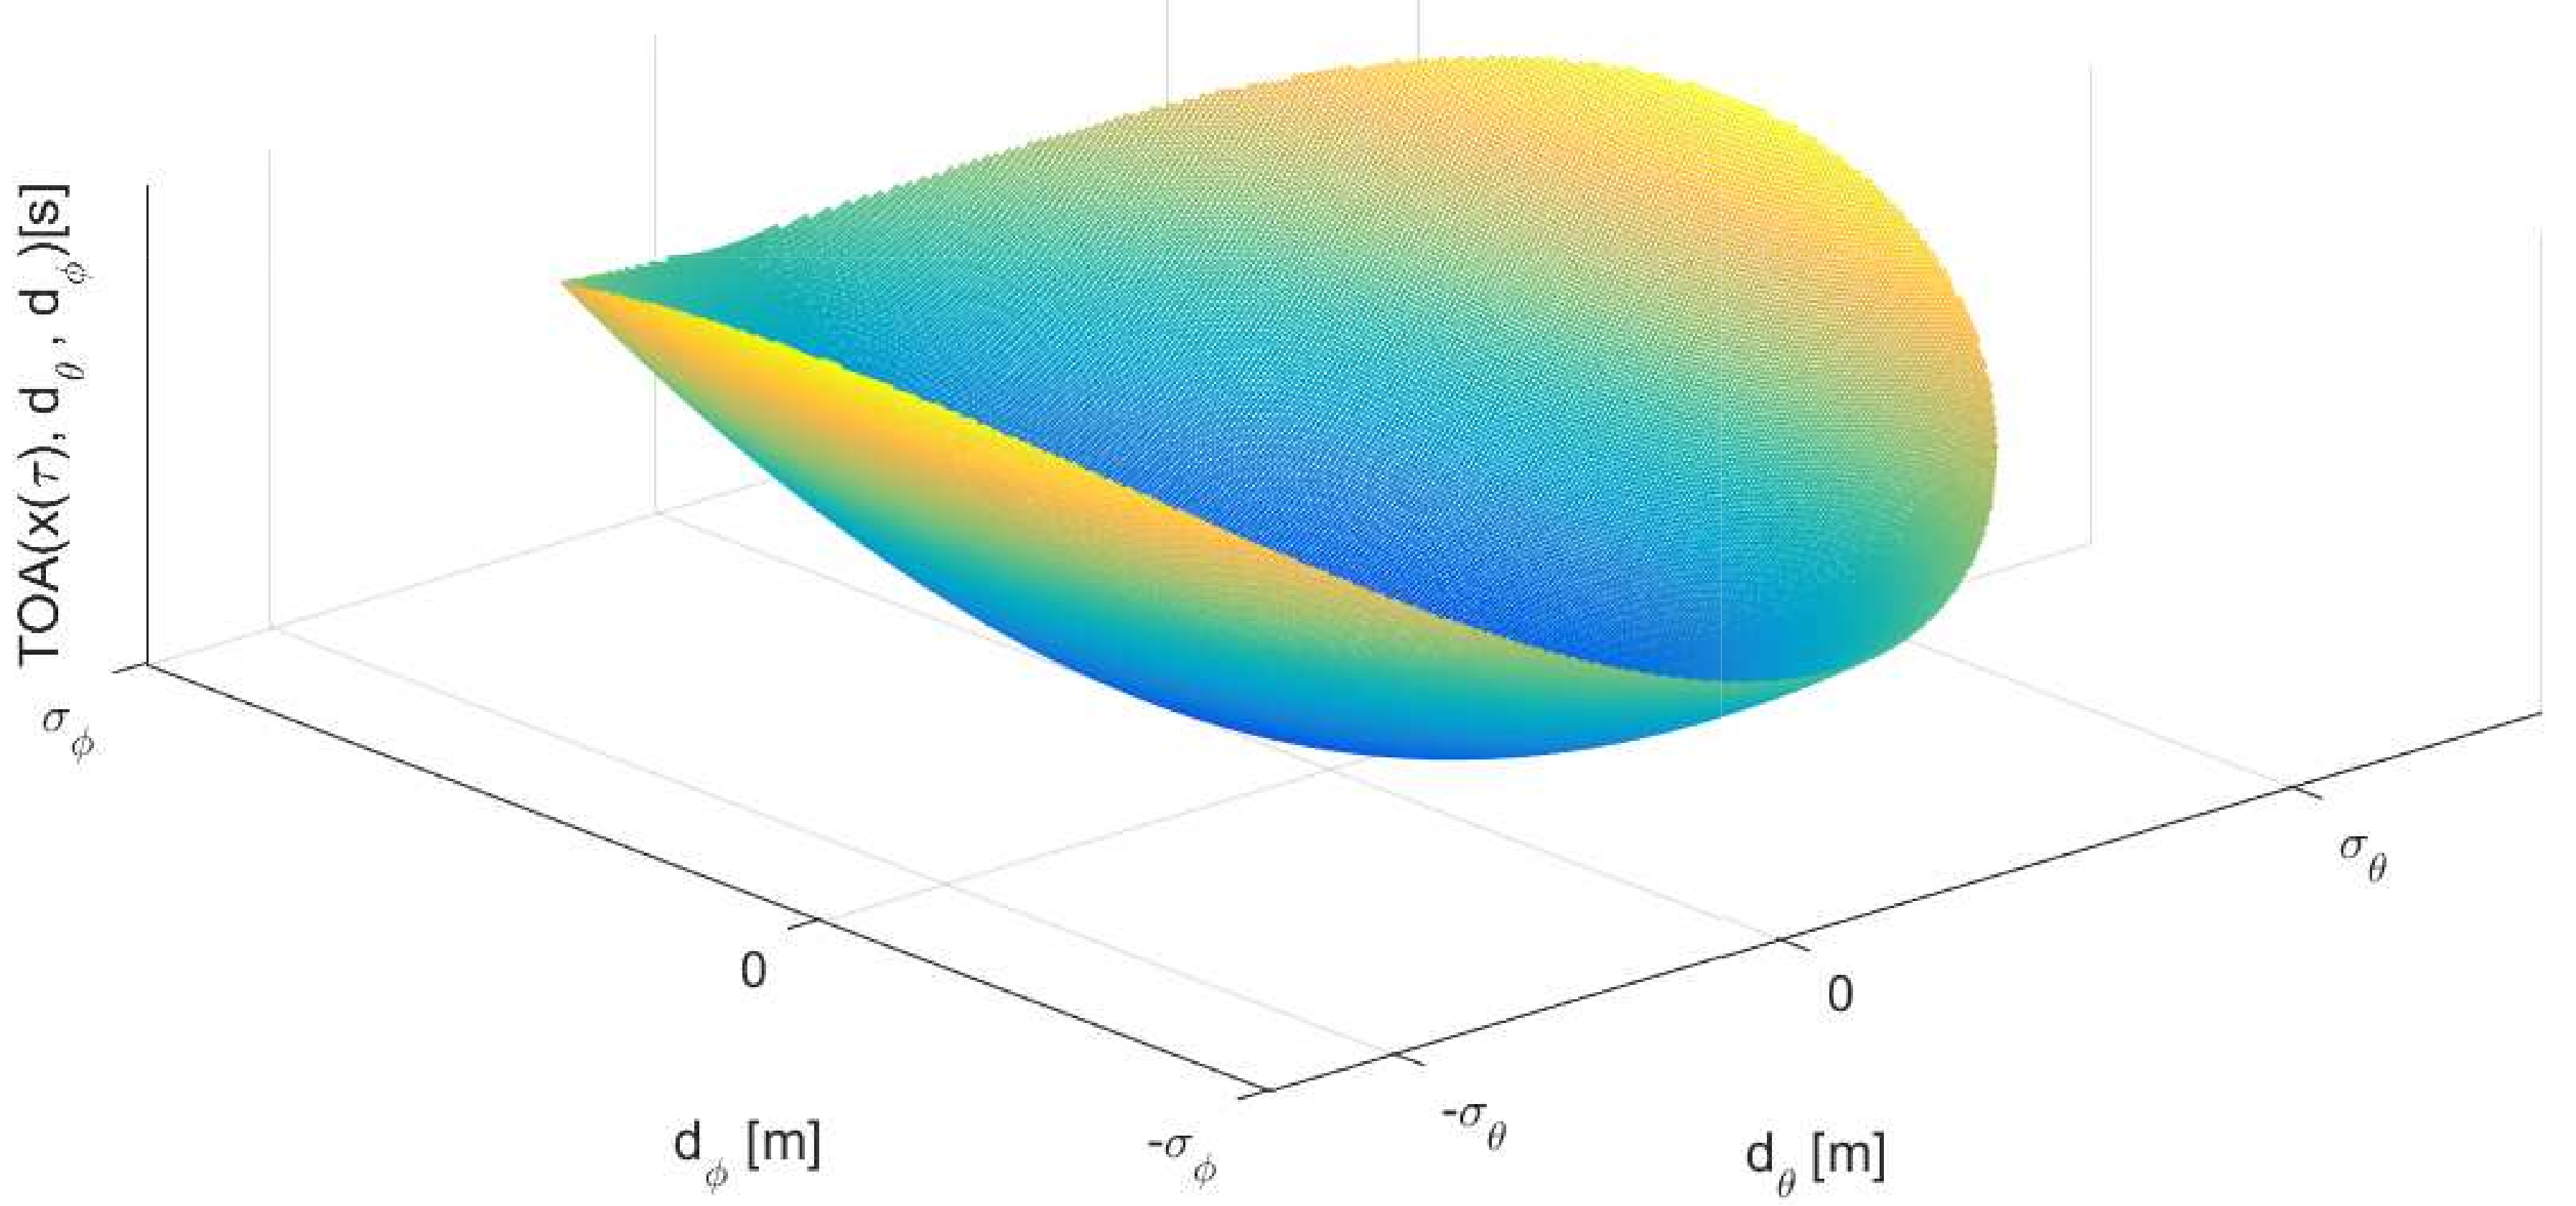
\includegraphics[width=0.7\textwidth]{\FIGDIR/TE016EllipsoidCutTimeOfArrival} 
    \caption{Time Of Arrival (TOA) for one ellipsoid $E_D({x}(\tau),{v})$.}
    \label{fig:intruderTimeOfArrival}
\end{figure}

\noindent The intersection rate $P_D({x}(\tau),c_{i,j,k},\theta,\varphi)$ for one time sample $\tau$ is given by (eq. \ref{eq:spreadIntersectionProbFixedtauDiscrete}), which has similar notation to (eq. \ref{eq:spreadIntersectionProbFixedtau}), sums are used instead of integrals and discrete rate density function $P_D({x}(\tau),d_\theta,d_\varphi,{p})$ for points form ellipse and cell intersection are used as iterator base set ${p}\in\left\{E_D({x}(\tau),{v})\cap c_{i,j,k}\right\}$.

\begin{equation}\label{eq:spreadIntersectionProbFixedtauDiscrete}
    P_D({x}(\tau),c_{i,j,k},\theta,\varphi) =\sum_{{p}\in \left\{E_D({x}(\tau),{v})\cap c_{i,j,k}\right\}} P_D({x}(\tau),d_\theta,d_\varphi,{p})
\end{equation}

\noindent The \emph{space intersection rate} $P_{TD}(i_k({x}_s,{v},\theta,\varphi),c_{i,j,k})$ (eq. \ref{eq:spreadIntruderIntersectionProbDiscrete}) is given as mean intersection rate of partial intersections $P_D({x}(\tau),c_{i,j,k},\theta,\varphi)$ where step set $T=\{$ $i_e(c_{i,j,k})$, $\dots$, $i_l(c_{i,j,k})\}$ contains all viable intersection times with ellipsoids $E({x}(\tau\in T),{v})$. The denominator is basically count of samples in sample time set $T$. 

\begin{equation}\label{eq:spreadIntruderIntersectionProbDiscrete} 
    P_{TD}(i_k({x}_s,{v},\theta,\varphi),c_{i,j,k})=\frac{\sum_{\tau=i_e(c_{i,j,k})}^{i_l(c_{i,j,k})} \sum_{{p}\in E_D({x}(\tau),{v})}P_D({x}(\tau),c_{i,j,k},\theta,\varphi,{p})}{\sum_{\tau i_l(c_{i,j,k})}^{i_e(c_{i,j,k})} 1}
\end{equation}

\noindent An \emph{intersection of intruder cone and cell} $c_{i,j,k}$ cell is defined by (eq. \ref{eq:conicIntersectionCellIntruderDiscrete}) The  set of point ${p}\in\mathscr{R}^3$ where condition of intersection between ellipsoids $E_D({x}(\tau),{v})$ for times $\tau\in\mathscr{R}^+$ and cell space $c_{i,j,k}$ is met.

\begin{equation}\label{eq:conicIntersectionCellIntruderDiscrete}
    \mathscr{P}(i_k({x}_s,{v},\theta,\varphi),c_{i,j,k})= \bigcup_{\forall \tau\in\mathscr{R}^+} \left\{{p}\in\mathscr{R}^3:{p}\in c_{i,j,k}\cap E_D({x}(\tau),{v})\right\}
\end{equation}

\noindent An \emph{intruder time of entry} $i_e(i_k,c_{i,j,k})$ (eq. \ref{eq:conicTimeOfEntryDiscrete}), for intruder $i,k$ and cell $c_{i,j,k}$ is approximated for discrete point set  $\mathscr{P}(i_k({x}_s,{v},\theta,\varphi),c_{i,j,k})$ (eq. \ref{eq:conicIntersectionCellIntruderDiscrete}) as minimal time of arrival $t_{TOA}({p})$ of member points ${p}$.

\begin{equation}\label{eq:conicTimeOfEntryDiscrete}
    i_e(i_k,c_{i,j,k})\approx \min \left\{t_{TOA}({p}):{p}\in\mathscr{P}(i_k({x}_s,{v},\theta,\varphi),c_{i,j,k})\right\}
\end{equation}

\noindent An \emph{intruder time of leave} $i_l(i_k,c_{i,j,k})$ (eq. \ref{eq:conicTimeOfLeaveDiscrete}), for intruder $i,k$ and cell $c_{i,j,k}$ is approximated for discrete point set  $\mathscr{P}(i_k({x}_s,{v},\theta,\varphi),c_{i,j,k})$ (eq. \ref{eq:conicIntersectionCellIntruderDiscrete}) as maximal time of arrival $t_{TOA}({p})$ of member points ${p}$.

\begin{equation}\label{eq:conicTimeOfLeaveDiscrete}
    i_l(i_k,c_{i,j,k})\approx \max \left\{t_{TOA}({p}):{p}\in\mathscr{P}(i_k({x}_s,{v},\theta,\varphi),c_{i,j,k})\right\}
\end{equation}

\paragraph{Combined intersection model:} The \emph{combined intersection model} $P_{O_I}(i_k,c_{i,j,k},l,b,s,\tau)$ is defined for intruder $i_k$ with parameters:

\begin{enumerate}
    \item\textit{Starting position} ${x}_s$ - expected position of intruder $i_r$ in 3D space at time of avoidance $t_i$ in avoidance grid frame $\mathscr{A}(t_i)$.
    
    \item\textit{Velocity vector} ${v}$ - oriented velocity of intruder $i_r$ at time of avoidance $t_i$ in avoidance grid frame $\mathscr{A}(t_i)$. 
    
    \item\textit{Horizontal uncertainty spread} $\theta$ - defines how much can intruder $i_r$ deviate on horizontal axis of intruder local coordinate frame (if X+ is main axis, then Y is horizontal axis in right-hand euclidean coordinate frame), due the properties of intersection definition, the horizontal uncertainty spread can have following values $\theta\in[0,\pi/2]$.
    
    \item\textit{Vertical uncertainty spread} $\varphi$ -defines how much can intruder $i_r$ deviate on vertical axis of intruder local coordinate frame (if X+ is main axis in local right-hand euclidean intruder coordinate frame, then Z is horizontal vertical axis), due the intersection definition, the vertical uncertainty spread can have following values $\varphi\in[0,\pi/2]$.
    
    \item\textit{Body volume radius} $r$ - defines the body volume of intruder in meters and it is having  $\R^+$  value.
\end{enumerate}

\noindent The \emph{flag vector} $l,b,s,\tau \in \left\{0,1\right\}$ is parametrization of rate calculation: $l$ stands for \emph{lined intersection}, $b$ stands for \emph{body intersection}, $s$ stands for \emph{spread intersection}, $\tau$ stands for \emph{time account}. 

The \emph{space intersection for line} $P_L(i_k,c_{i,j,k})$ is defined as $P_T(i_k({x},{v}),c_{i,j,k})$, where $i_k$ is intruder with properties of initial position ${x}$, velocity vector ${v}$ and $c_{i,j,k}$ is target cell. (eq. \ref{eq:baseIntersectionProbabilityLineIntersectionType}). 

The \emph{space intersection rate for body volume} $P_B(i_k,c_{i,j,k})$ is defined as $P_T(i_k({x},{v},r),c_{i,j,k})$ (eq. \ref{eq:baseIntersectionProbabilityBallIntersectionType}), where intruder $i_r$ has additional property of the intruder body volume radius $r$. 

The \emph{space intersection probability for maneuverability uncertainty} $P_S(i_k,c_{i,j,k})$ is defined as $P_{TD}(i_k({x}_s,{v},\theta,\varphi),c_{i,j,k})$ (eq. \ref{eq:spreadIntruderIntersectionProbDiscrete}), where intruder properties $\theta$, $\varphi$ stands for intruder horizontal and vertical uncertainty spread.

The \emph{time intersection rate} $P_{\tau,x}(i_k,c_{i,j,k})\in[0,1]$ is defined in (eq. \ref{eq:intruderIntersectionProbability}). This probability has two calculation modes, first is for 1D intersection (line), second is for volume intersection (body volume, spread elliptic cone).  

UAS cell entry time $t_e$ and cell leave time  $t_l$ time for vehicle in avoidance grid $\mathscr{A}(t_i)$ are given by (eq. \ref{eq:cellEntryTime}) and (eq. \ref{eq:cellLeaveTime}). 

Intruder leave and entry time for 1D intersections is trivial and is omitted in this section. Intruder entry $i_e$ and intruder leave $i_l$ for 3D intersection are given by (eq. \ref{eq:conicTimeOfEntryDiscrete}, \ref{eq:conicTimeOfLeaveDiscrete}). 

All partial rates with respective definition references are summarized in (eq. \ref{eq:partialProbabilitiesIntruderSummary})

\begin{equation}\label{eq:partialProbabilitiesIntruderSummary}
    \begin{aligned}
        P_L(i_k,c_{i,j,k}) &= P_T(i_k({x},{v}),c_{i,j,k}) &(\ref{eq:baseIntersectionProbabilityLineIntersectionType})\\
        P_B(i_k,c_{i,j,k}) &= P_T(i_k({x},{v},r),c_{i,j,k}) &(\ref{eq:baseIntersectionProbabilityBallIntersectionType})\\
        P_S(i_k,c_{i,j,k}) &= P_{TD}(i_k({x}_s,{v},\theta,\varphi),c_{i,j,k}) &(\ref{eq:spreadIntruderIntersectionProbDiscrete})\\
        P_{\tau,x}(i_k,c_{i,j,k})&=\frac{\norm{[i_e(c_{i,j,k}),i_l(c_{i,j,k})]\cap [t_e,t_l]}}{\norm{[t_e,t_l]}}& (\ref{eq:intruderIntersectionProbability})\\
    \end{aligned}
\end{equation}

\noindent With definition of all space and time intersection rates (eq. \ref{eq:partialProbabilitiesIntruderSummary}) and given flag vector $l,b,s,\tau \in\left\{0,1\right\}$ one can formulate combined intersection rate $P_{O_I}(i_k,c_{i,j,k},l,b,s,\tau)$ (eq. \ref{eq:intruderInCellProbabilityOneIntruder}) for intruder $i_k$ and cell $c_{i,j,k}$. The principle is following: \emph{maximum of selected rates product based on flag vector is final intersection rate of intruder $i_k$ in cell}. 

The time-use flag $\tau$ is adding time intersection rate $P_{\tau,x}(i_k,c_{i,j,k})$, where time intersection rate is defined by $x=\left\{L,B,S\right\}$ for line, body volume, spread ellipse time intersections ($P_{\tau,L}(i_k,c_{i,j,k})$ $\neq$ $P_{\tau,B}(i_k,c_{i,j,k})$ $\neq$ $P_{\tau,B}(i_k,c_{i,j,k})$ for one intruder $i_k$).

\begin{equation}\label{eq:intruderInCellProbabilityOneIntruder}
    \begin{aligned}
        P_{O_I}(i_k,c_{i,j,k},l,b,s,\tau) & = \begin{cases}\tau=0&:\max\left\{\begin{aligned}P_L(i_k,c_{i,j,k}).l\\ P_B(i_k,c_{i,j,k}).b\\P_S(i_k,c_{i,j,k}).s\end{aligned}\right\}\\\tau=1&:\max\left\{\begin{aligned}P_{\tau,L}(i_k,c_{i,j,k}).P_L(i_k,c_{i,j,k}).l\\ P_{\tau,B}(i_k,c_{i,j,k}).P_B(i_k,c_{i,j,k}).b\\P_{\tau,S}(i_k,c_{i,j,k}).P_S(i_k,c_{i,j,k}).s\end{aligned}\right\}\end{cases} &\\
    \end{aligned}
\end{equation}